\glsresetall

\emph{In situ} Data Exploration is an active research area that requires
a multidisciplinary approach: algorithms, data structures, machine learning,
statistics,  data visualization, information sciences, and, unavoidably,
the domain knowledge --- or business understanding ---  provided by an expert.

Going back to the \gls{CRISPDM} model described in  chapter~\ref{chapter:introduction}
and shown in figure~\ref{fig:crispdm}, our initial objective was to identify
gaps in the tooling available for experts to understand data coming as a set of
unprocessed and perhaps inconsistent set of files. These files are not optimized
for access, and any early decision on how to ingest them into a database may be
counterproductive until the dataset is better understood.

The literature survey from chapter~\ref{chapter:literature_review} showed that
solutions for visualization, optimizations, indexing, storage,\ldots abound.
Still, there is little to no mention of assisting users on \emph{understanding}
data schema, especially when it comes to multiple files from diverse origins or
when meta-data is incomplete or inconsistent.
In chapter~\ref{chapter:diverse}, we have seen that users spend a non-negligible
amount of resources just examining the data structure and layout.

The question that followed was: can we leverage the data \emph{distribution} to
assist users in understanding the schema, on seeing how different datasets may come together?
This is particularly important when the data is numerical and uncertain since
one can not just compare tuples individually but needs to inspect distributions.

In the relational world, the \gls{IND} concept comes close to the objective:
parts of a relation contained (included) within another. However, this modeling
relies on the attributes' discrete nature, such as name, date of birth, etc.

In chapter~\ref{chapter:presq} we propose a generalization, the \gls{EDD}, that
relaxes the strict containment relation required by \glspl{IND}.
We then introduce \PresQ, a novel algorithm for \gls{EDD} finding that incorporates
uncertainty into its world modeling, proving that relying on data distribution alone is feasible.
Therefore, \PresQ is applicable in situations where most existing \gls{IND} solutions
are not: when the data is intrinsically uncertain --- measures of physical properties ---,
or when the validation strategy for the inclusion is an approximate heuristic.
The only requirement is that the expectation of false negatives --- i.e., significance
level for statistical tests --- can be estimated.

For the experiments used to evaluate \PresQ, described in ~\ref{sec:presq_experiments},
the statistical test of choice was based on the $k$-nearest neighbors. While this test
performs well for a wide range of datasets, the resulting trained \emph{model} is not
very useful.
Chapter~\ref{chapter:som} introduces a statistical test based on \gls{SOM}, which provides,
in addition to a $p$ value, a trained projection that we can later use for binning and
cross-matching both datasets using the matching set of features. The resulting \gls{SOM}
is also interpretable in case of rejection, which is also helpful in tentative data exploration.

\section{Future work}
\todo{Is it worth to mention dead-ends? i.e., structure on Probabilistic Graphical Networks}

\begin{itemize}
    \item In chapter~\ref{chapter:presq}, we prove that finding quasi-cliques in hypergraphs
    is a successful technique to find \gls{EDD}, or \gls{IND} based on approximate heuristics
    between relations. Therefore, a place for further research is to
    \textbf{improve the quasi-clique finding} algorithm, either via novel algorithms or by
    generalizing some of the many existing techniques~\cite{WU2015693}.
            
    \item On the other hand, the existing algorithms based on quasi-clique search forget
    about certain aspects of the datasets. For instance, the correlation matrix on both
    sides of the \gls{EDD} is likely to be similar, and it may be possible to leverage
    \textbf{data-aware} algorithms to augment the quasi-clique finding.
    
    \item Sometimes, the algorithms should not assume equality-of-distribution. For instance, one of the
    datasets may have been filtered beforehand --- i.e., signal-to-noise, value clipping, etc. This issue affects
    both \gls{EDD} and \gls{IND} algorithms~\cite{koeller2003discovery}. \textbf{Partial inclusion/equality-of-distribution}
    remains an open problem.
            
    \item \PresQ is based on frequentist probability, which does not allow incorporating \textbf{prior beliefs}
    into the algorithm. i.e., a \textbf{domain-expert} has no way of influencing the result based
    on her knowledge of the area.
    A Bayesian framework could prove helpful in this respect. Furthermore, in relation with the previous point,
    it can also be used to perform local null hypothesis testing~\cite{soriano2015bayesian}, which could help
    identify partial \glspl{EDD} --- as when a filter has been applied to one of the datasets.
    
    \item Searching for quasi-cliques involves exponential time complexity on the number of nodes.
    Thus, beforehand, applying a \textbf{dimensionality reduction} would reduce the total
    run-time and decrease the noise. Nonetheless, a complication arises from the premise that
    we do not know which attributes are shared.
        
    \item Finally, \textbf{finding other types of numerical dependencies} can be of interest.
    For instance, a single dataset may be split between multiple files based on the values
    from a given set of attributes, which may or may not overlap.
    As an example, figure~\ref{subfig:tu_multifile} shows an example where a single dataset is
    cleanly cut using two spatial dimensions, which can be easily \emph{learned} by a decision tree.
    Figure~\ref{subfig:mer_multifile} shows another dataset also cut using the same two
    coordinates, but where there exists an overlap between some of the files.
\end{itemize}

\begin{figure}[htbp]
    \begin{subfigure}[]{0.5\textwidth}
    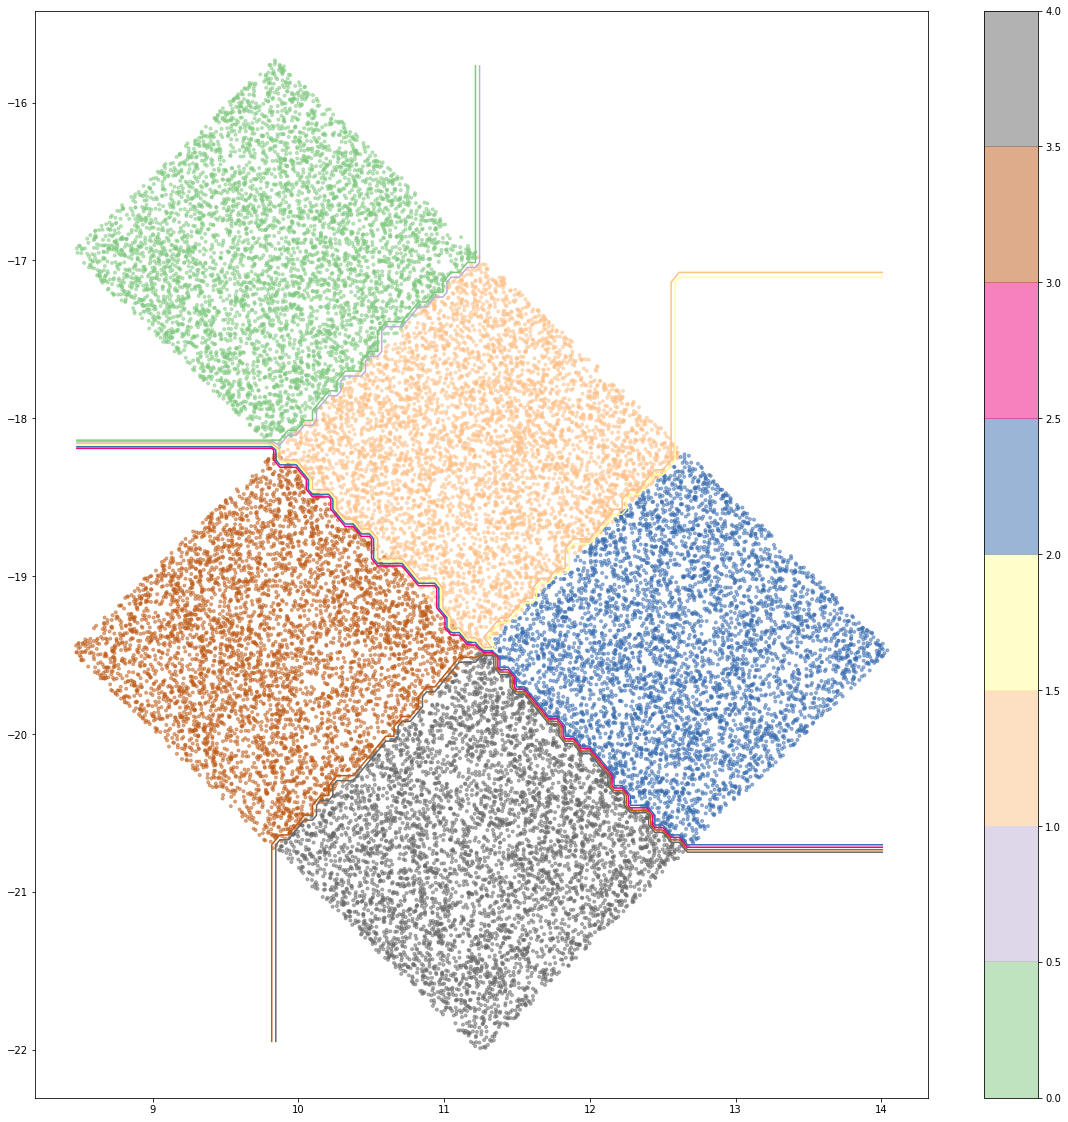
\includegraphics[width=\textwidth]{images/6_conclusions/tu_multifile_tree.png}
    \caption{Without overlap}\label{subfig:tu_multifile}
    \end{subfigure}
    \hfill
    \begin{subfigure}[]{0.5\textwidth}
    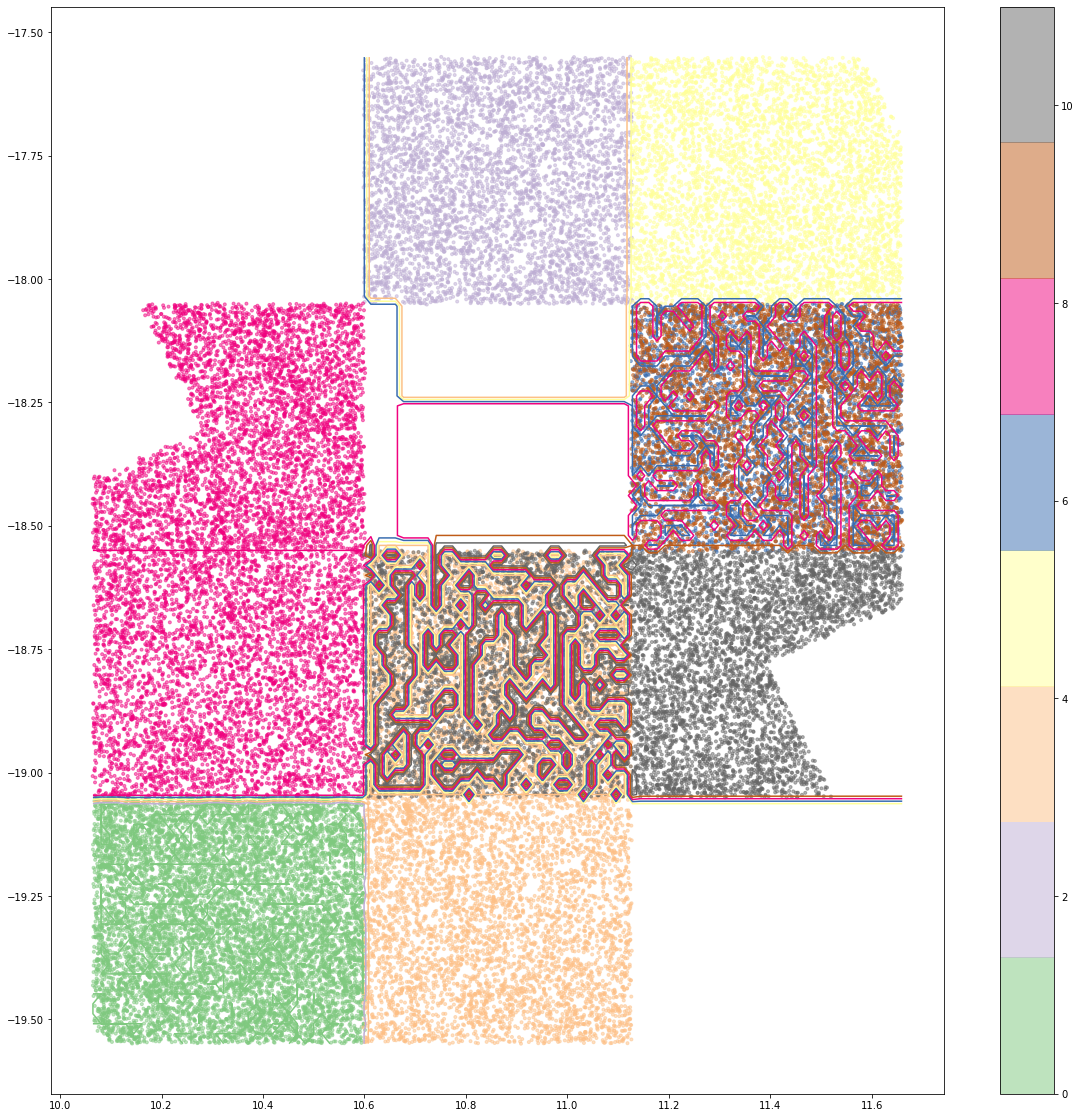
\includegraphics[width=\textwidth]{images/6_conclusions/mer_multifile_tree.png}
    \caption{With overlap}\label{subfig:mer_multifile}
    \end{subfigure}
    \caption{
        Data-sets distributed multiple files based on two spatial coordinates.
        Each color corresponds to a single file.
    }
    \label{fig:tree_cat_cut}
\end{figure}
